% http://www.idsc.ethz.ch/education/theses-semester-projects.html
% IDSC LaTeX Thesis Template
% 
% Author(s):	Eric Müller
% 				Institute for Dynamic Systems and Control
% 				Swiss Federal Institute of Technology (ETH) Zurich
% 
% Created:		2004/04/02  (Eric Mueller)
% 
% Notes: Has been tested on Windows 7 + MikTeX + TeXnicCenter
%
% Revisions: 	2009/05/29  (Soren Ebbesen)
% 				    2011/03/22	(Soren Ebbesen)
%             2013/03/08	(Soren Ebbesen)
%             2014/03/13	(Soren Ebbesen)
% ______________________________________________________________________________
\documentclass[12pt,oneside,a4paper,fleqn]{article}
\usepackage{siunitx}
%\usepackage[utf8]{inputenc}
\usepackage[onehalfspacing]{setspace}
%\usepackage{lineno}\linenumbers

% CHANGE HERE FOR GERMAN (german) OR MASTER THESIS (mt)!!!!!

\usepackage[english,bt]{ethidsc} % Special IDSC styles and commands      	
								 % {german}/english: language of headings, etc.
								 % {st}/bt/mt: {semester}/bachelor/master thes
\addbibresource{references.bib}
\documentclass{report}
\usepackage{calligra}
\usepackage{mathtools}
\usepackage{amsmath}
\usepackage{float}
\usepackage{siunitx} 
\usepackage{array}
\usepackage{hyperref}
\usepackage{graphicx}
\usepackage{booktabs}
\usepackage{geometry}
\usepackage{subcaption}
\usepackage{amssymb}
\usepackage{microtype}
\usepackage{braket}

% Page header (don't change)____________________________________________________
\setlength{\parindent}{0em}                 % Disable parindent
\rhead[\nouppercase{\rightmark}]{\thepage}  % Special headings
\lhead[\thepage]{\nouppercase{\leftmark}}   % Special headings
\cfoot{}                                    % Special headings


% Title page (please fill in)___________________________________________________
\title{Influence of probabilistic abstention on spatial cooperative games}


\studentA{Alessandro Azzani, Francesco Gargiulo \\ Lea Haas}
%\ethidA{20-000-00}
%\semesterA{6}
%\emailA{someone@student.ethz.ch}

\studentB{Nicol\`{o} Montalti}
%\ethidB{12-345-678}
%\semesterB{9}
%\emailB{second@student.ethz.ch}

%\supervision{Prof. Dr. Superviser}
\date{\today}

%\identification{IDSC-XX-YY-ZZ} 		% Project identifier

%\infopage
%\declaration

% Begin document________________________________________________________________
\begin{document}

\maketitle 							% Create title page

\pagenumbering{roman}
\tableofcontents
\newpage
% Preamble______________________________________________________________________

%\pagenumbering{roman} 				% Begin roman page numbering (i,ii,...)

%\input{chapters/preamble} %Abstract etc.

% Chapters______________________________________________________________________

\pagestyle{fancy}               	% Fancy headings			
\setlength{\parindent}{20pt}

% We start writing from here -----------------------------------------------------
\addcontentsline{toc}{section}{Individual contributions}
\section*{Individual Contributions}
\label{chap:indv}

Who did what....

\newpage
\addcontentsline{toc}{section}{Introduction}
\section*{Introduction}
\pagenumbering{arabic}

\label{chap:intro}

Here we write the introduction.
% what was our plan


\section{Theoretical background}
\subsection{Game theory}
\subsection{Games}
%PD, SH, HG, SD
\subsection{Spatial games}
% repeated games, imitation

\subsection{Abstention}
% optional abstention, probabilistic abtention (PD, OPD, PDPA)
% (paper: DOI:10.1038/s41598-018-32933-x)

\section{Implementation}
The game has been implemented in Python, the code is publicly available on GitHub \cite{montalti2023}. The spatial environment has been implemented as a $50 \times 50$ 2D grid. A player is present at every point of grid. Every player is characterized by a strategy (collaborate / defect) and by an abstention probability $0 \leq \alpha \leq 1$. The game is defined by the five parameters $T, R,  P, S, L$ and by a noise factor $0 \leq \eta \leq 1$. The first five parameters determine the game played: prisoner dilemma (PD), snowdrift (SD), stag hunt (SH) or harmony game (HG).

The game is initialized assigning to each player a random strategy, with a $50-50$ probability, and an abstention probability $\alpha$. The latter can be assigned in three different ways:
\begin{itemize}
    \item No abstention: $\alpha = 0$ for all players. The game is reduced to the standard prisoner dilemma (PD) or another standard game
    \item Optional abstention: $\alpha = 0$ or $1$ with a $50-50$ probability. The game is reduced to the optional prisoner dilemma (OPD) or the equivalent for another game
    \item Probabilistic abstention: $\alpha \in [0,1]$. The players have a finite probability of absteining, uniformly distributed between 0 and 1. We call this situation prisoner dilemma with probabilistic abstention (PDPA) or the equivalent for other games.
\end{itemize}

At each iteration of the game, each player plays against their four nearest neighbours. Each player earns an amount equal to the sum of the payoff of the four games they played. The payoff of a single match between two players is determined by the strategy of the two players and by their abstention probability. Each player joins the game with a probability $1-\alpha$. If both players join the game, the game is played and payoffs are distributed according to the players strategies. If one of the players abstains, the game is not played, and both players receive a payoff $L$.

After every player has played, the imitation process begins. The imitation process is influenced by the noise parameter $\eta$. Each player changes their strategy to the opposite strategy with a probability $\eta$ and imitates their best performing neighbours with a probability $1-\eta$. If the imitation option is chosen, the player looks at their four nearest neighbours payoffs, and imitates the strategy of the one who performed the best. If more players share the same optimal outcome, a random one is chosen. In addition to imitating the best-performing player's strategy, the abstention probability is imitated as well.

The process is iterated for a fixed number of times $t$ (usually $t=200$). At each iteration, the players play the game and imitate their neighbours' strategies and abstention probabilities. At the end of the cycle, some statistics are extracted from the final configuration. Taking inspiration from Cardinot \emph{et al.} \cite{cardinot2018} we evaluate the mean abstention probability $\langle \alpha \rangle$ and the mean the effective cooperation frequency $\varepsilon = (1-\alpha)\cdot (1-s)$, where $s = 0$ for a cooperator and $s=1$ for a defector. In addition to these two quantities, we also analyse the correlation between being a cooperator and having a low abstention frequency $\alpha$. To do so, when playing the version of the game with probabilistic abstention, we plot the number cooperators and defectors for each value of $\alpha$ and compare the results.
%Quante run avete fatto? 10 ok, aggiungo anche gli altri giochi? Direi di sì. Snow drift è abbastanza interessante visto che c'è un comportamento particolare per T > 1.6, per gli altri si può dire che non c'è una grande differenza. Allora genero i grafici prima per snow drift, al massimo mettiamo anche per gli altri e sottolineiamo che non succede nulla di interessante, ma almeno lo facciamo vedere. Aspetta io intendo le Figure 3, 4, 5. Te cosa vuoi generare? La correlazione? Ah non avevo visto che le figure già facessero riferimento ai diversi giochi. Avevo visto per ora solo quella di pd. Ok, poi se vuoi generare qualcosa che ti viene in mente ovviamente puoi giocare un po' col codice. Si si nel caso se penso che possa servire in aggiunta a quello che abbiamo già

\section{Results}
First of all we start by comparing the results we derive with the ones obtained by \cite{cardinot2018} for the dependence of effective cooperation frequency on the temptation payoff the with the ones we obtain: 
\begin{figure}[H]
    \centering
    \subfloat[]{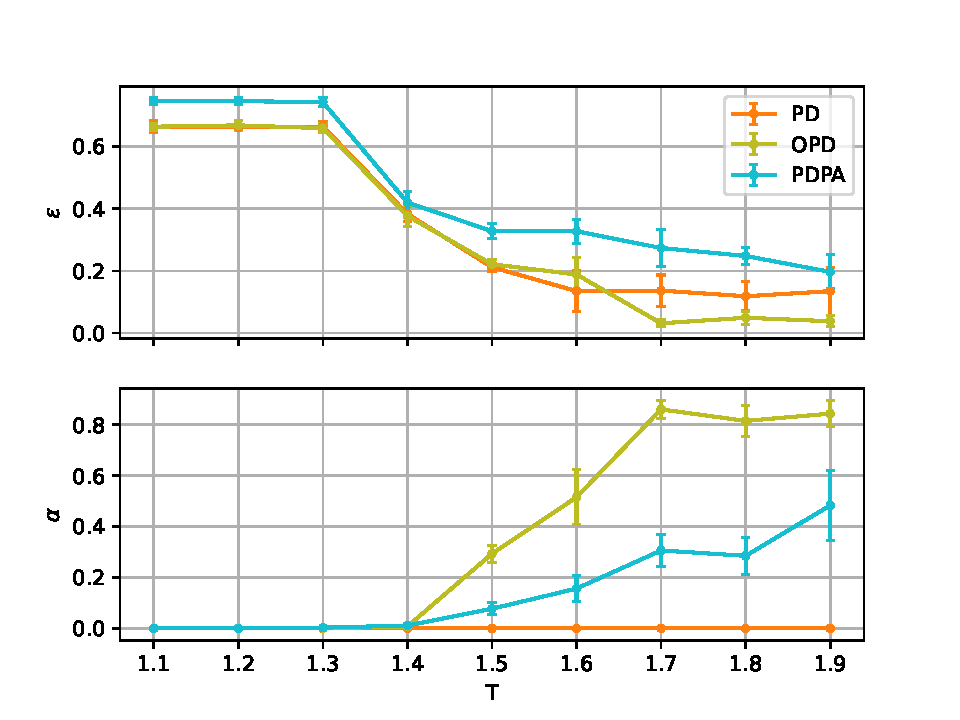
\includegraphics[scale = 0.5]{Images/alpha_eps-20230606-125503.pdf}}
    \subfloat[]{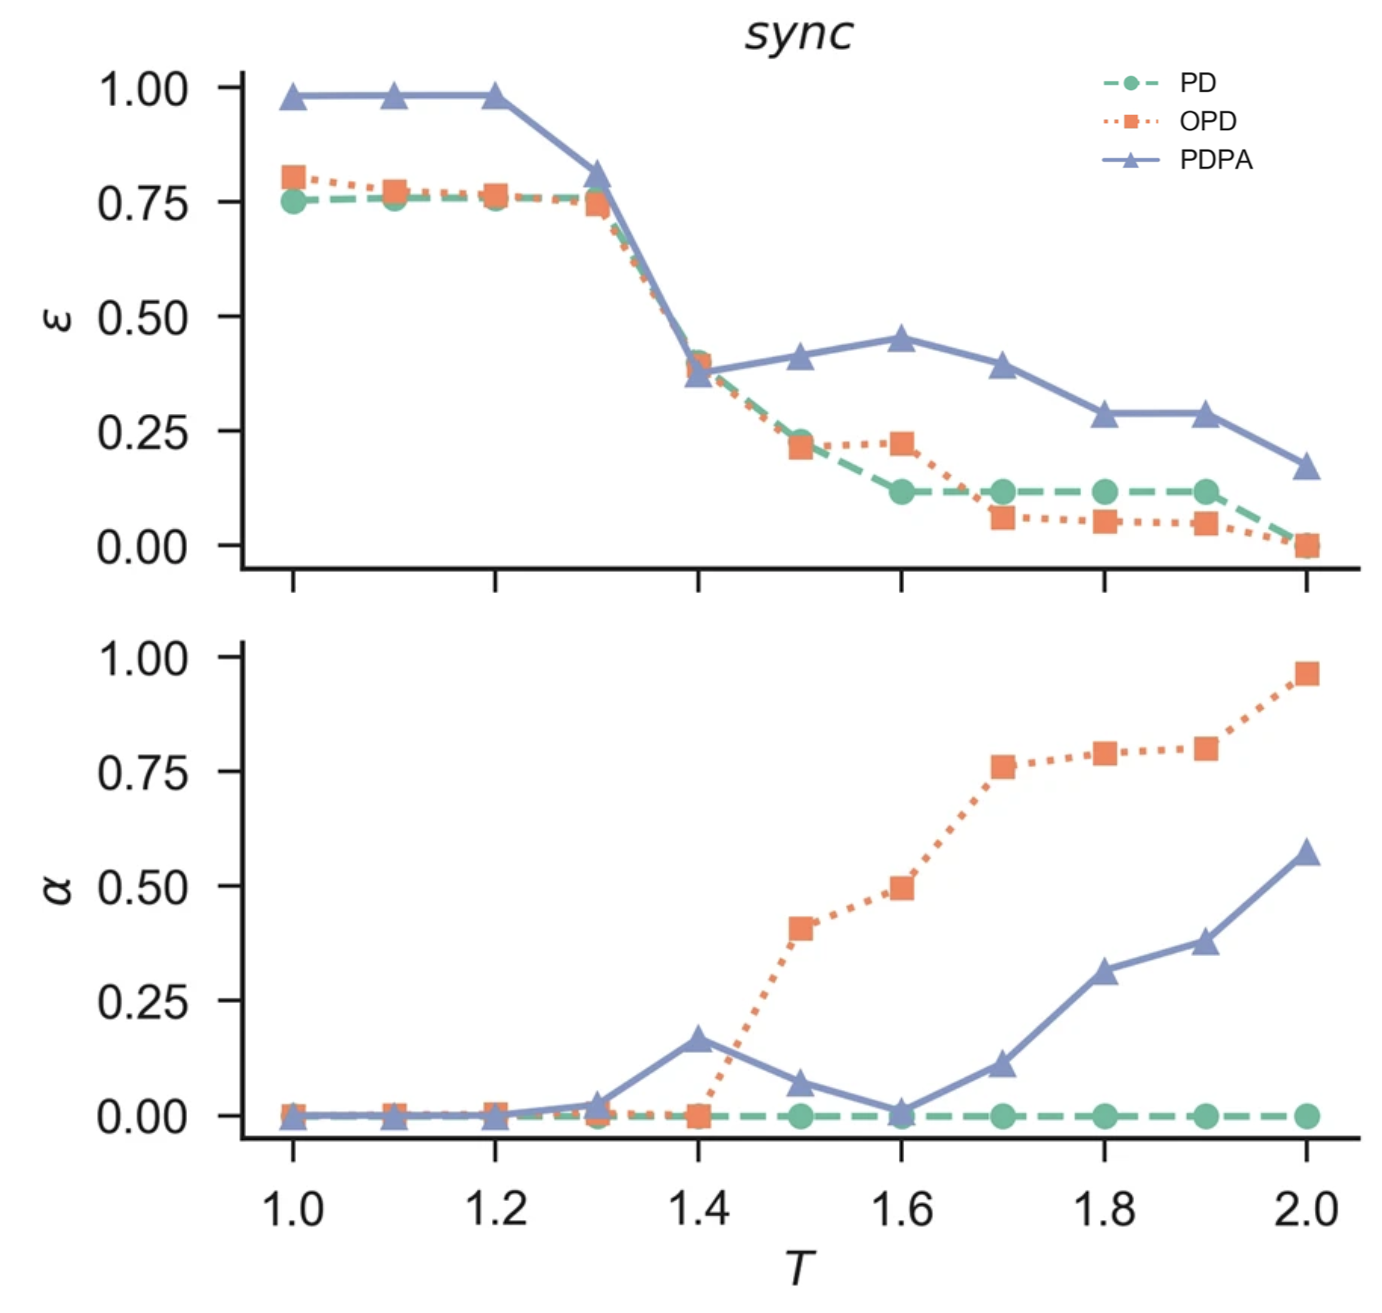
\includegraphics[scale = 0.23]{Images/dependence of alpha and epsilon on T.png}}
    \caption{(a) shows the dependence we obtained for $\alpha$ and $\epsilon$ on T where we set R = 1 S = 0 P = 0.3 L = 0.4 noise = 0.001 t = 200. The results are obtained after averaging 10 runs (b) correspond to the results obtained from Cardinot et Al \cite{cardinot2018}.}
    \label{fig: comparison of epsilon and alpha}
\end{figure}
Once we have made sure that the results are compatible with the ones derived we proceed to analyze the other possible games. We start by looking at snowdrift 

\begin{figure}
    \centering
    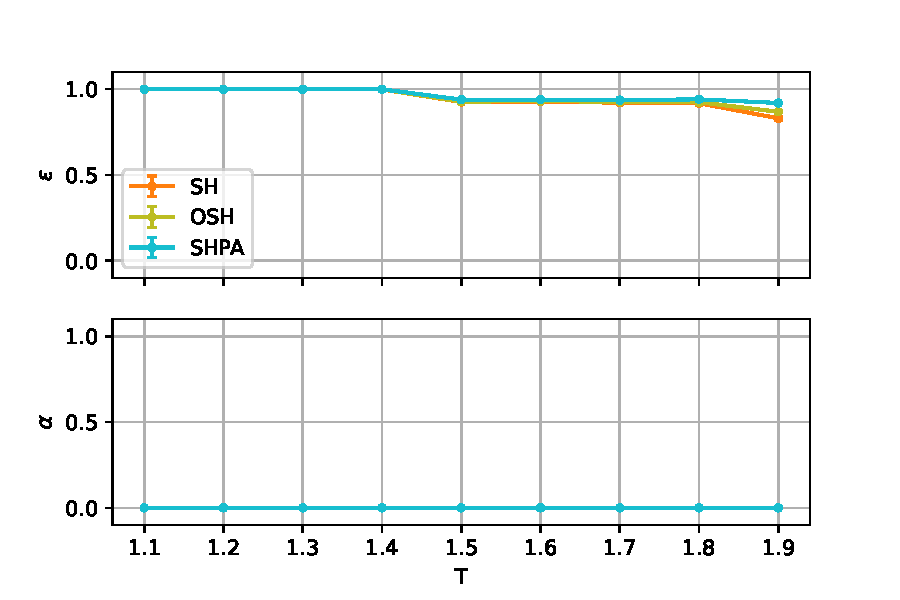
\includegraphics{Images/alpha_eps-20230606-124900.pdf}
    \caption{R = 1
        S = 0
        P = 0
        L = 0.4
        noise = 0.001
        t = 200}
    \label{fig:enter-label}
\end{figure}

\begin{figure}
    \centering
    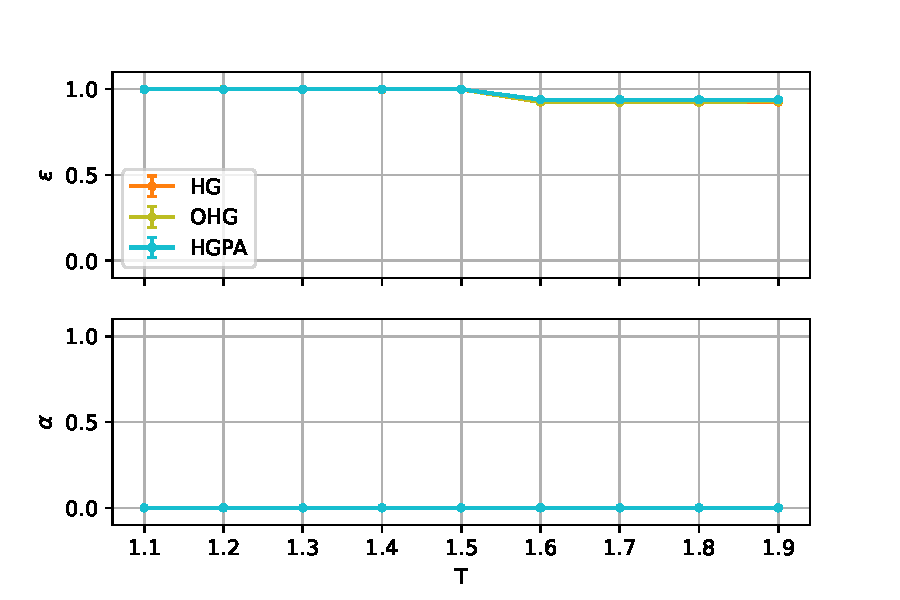
\includegraphics{Images/alpha_eps-20230606-130744.pdf}
    \caption{R = 2
        S = 0.3
        P = 0
        L = 0.4
        noise = 0.001
        t = 200}
    \label{fig:enter-label}
\end{figure}

\begin{figure}
    \centering
    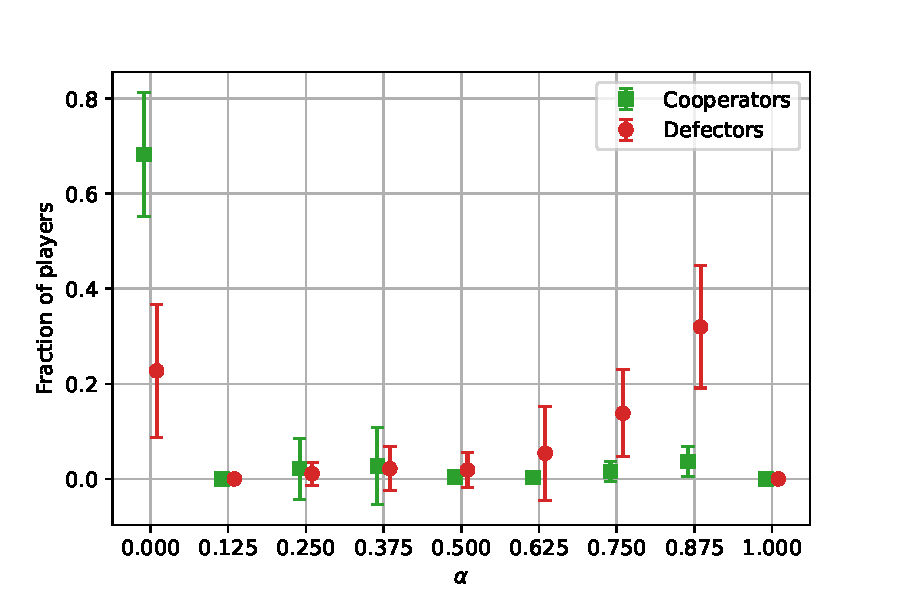
\includegraphics{Images/alpha.pdf}
    \caption{Correlation between abstention and cooperation. For each value of $\alpha$, the relative number of cooperators is compared to the relative number of defectors. The numbers are normalized dividing by the total number of players. The marks of cooperators (defectors) are slightly shifted to the left (right) for better readability. Parameters: $T = 1.4, R = 1, S = 0, P = 0.3, L = 0.4$}
    \label{fig:enter-label}
\end{figure}

\section{Conclusions}

% Bibliography__________________________________________________________________
% Literature (Additional references can be added to the .bib-file manually, or by using, for example, the free application JabRef). Compile in the following order: latex -bibtex -latex -latex

%\bibliographystyle{plain}
%\begin{footnotesize}
%    \bibliographystyle{apalike}
%    \bibliography{references}
%\end{footnotesize}

\newpage

\printbibliography
\end{document}
